\documentclass{article}
\usepackage{amssymb} % Required for math symbols
\usepackage{graphicx} % Required for inserting images
\usepackage{hyperref}
\usepackage{float}
\usepackage{bibentry}

\usepackage[utf8]{inputenc}
\usepackage{amsmath}
\usepackage[a4paper, total={6in, 10in}]{geometry}

\title{Sistema de revision de codigo de estudiantes y propuesta de mejoras al codigo usando AI Generativa}
\author{anonymus@gg.pe}
\date{\today}

\begin{document}

\maketitle

\newpage
\tableofcontents
\newpage

% - Encontrar tecnicas de Machine Learning aplicadas a la revision de codigo en escuelas y/o universidades
% - Encontrar herramientas de Machine Learning aplicadas a la revision de codigo en escuelas y/o universidades
% - Encontrar experimentos similares
% - Encontrar como se validaria"



\section{Papers}

\subsection{"AICodeReview: Advancing code quality with AI-enhanced reviews" \cite{ALMEIDA2024101677}}

\textbf{Abstract:} This paper presents a research investigation into the application of Artificial Intelligence (AI) within code review processes, aiming to enhance the quality and efficiency of this critical activity. An IntelliJ IDEA plugin was developed to achieve this objective, leveraging GPT-3.5 as the foundational framework for automated code assessment. The tool comprehensively analyses code snippets to pinpoint syntax and semantic issues while proposing potential resolutions. The study showcases the tool's architecture, configuration methods, and diverse usage scenarios, emphasizing its effectiveness in identifying logic discrepancies and syntactical errors. Finally, the findings suggest that integrating AI-based techniques is a promising approach to streamlining the time and effort invested in code reviews, fostering advancements in overall software quality \cite{ALMEIDA2024101677}. \\

\textbf{Desglose:}

\begin{itemize}
    \item \textbf{Contexto:} La revisión de código es una práctica crítica en el desarrollo de software, destinada a garantizar la calidad del código y mejorar la colaboración en equipo. Sin embargo, el proceso de revisión manual puede ser lento y propenso a errores humanos. Este trabajo investiga la aplicación de la IA en las revisiones de código para mejorar su eficiencia y eficacia \cite{ALMEIDA2024101677}.
    
    \item \textbf{Research Gap/Problema:} A pesar del uso generalizado de las revisiones de código, los métodos manuales a menudo carecen de consistencia y son vulnerables a errores humanos. Las herramientas actuales de revisión automática de código no siempre proporcionan la profundidad necesaria para detectar problemas complejos, como los \textit{code smells}, que pueden afectar la calidad del software \cite{ALMEIDA2024101677}.
    
    \item \textbf{Hallazgos/Research Fill:} El estudio encontró que el uso del plugin desarrollado para IntelliJ, \textit{AICodeReview} (GPT-3.5 wrapper), es más efectivo que la revisión manual en la identificación y refactorización de \textit{code smells}. Esto sugiere que la integración de técnicas basadas en IA puede mejorar significativamente la calidad del código y la confiabilidad del software \cite{ALMEIDA2024101677}.
    
    \item \textbf{Limitaciones:} La evaluación preliminar de \textit{AICodeReview} se realizó con estudiantes de pregrado, lo que no representa a desarrolladores profesionales, pero el mismo experimento se puede realizar en un grupo profesional y uniforme en sus capacidades. Además, el estudio se centró en un conjunto limitado de \textit{code smells} y no incluyó una comparación exhaustiva con otras herramientas de revisión automática de código \cite{ALMEIDA2024101677}.
    
    % \item \textbf{Datasets:}
    
    \item \textbf{Métricas:} Se emplearon métricas como el tiempo de revisión, la cantidad de \textit{code smells} detectados y refactorizados, y la efectividad de la herramienta en la mejora de la calidad del código. El tamaño del efecto de Cohen (\textit{Cohen's d}) se utilizó para analizar las diferencias entre los grupos experimental y de control \cite{ALMEIDA2024101677}.
\end{itemize}

\textbf{Keypoints:}

\begin{itemize}
    \item \textbf{Técnica de ML/DL aplicada:} Se desarrollo un plugin para Intelligence que usa GPT3.5 por detrás, el código está disponible en \href{https://github.com/ElsevierSoftwareX/SOFTX-D-23-00603}{GitHub}.
    
    \item \textbf{Metodología:} Se dividió a los participantes en dos grupos: uno usando la herramienta \textit{AICodeReview} y otro realizando revisiones manuales. Se analizaron segmentos de código con aproximadamente 30 tipos diferentes de \textit{code smells} para comparar la efectividad de ambos métodos \cite{ALMEIDA2024101677}.
    
    \item \textbf{Experimentos:} La evaluación empírica involucró a 12 estudiantes de pregrado con conocimientos básicos de programación en Java y experiencia en el uso de IntelliJ IDEA. Se les capacitó en el uso de la herramienta antes de realizar las tareas de revisión \cite{ALMEIDA2024101677}.
    
    \item \textbf{Validación:} La validez interna del estudio se mantuvo mediante la división estratégica de los participantes y el establecimiento de un nivel de competencia base a través de sesiones de capacitación. Se emplearon métricas de validez concluyente, como el tiempo de revisión y el número de \textit{code smells} detectados y refactorizados \cite{ALMEIDA2024101677}.
\end{itemize}

You can find the paper \href{https://www.sciencedirect.com/science/article/pii/S2352711024000487}{here}.

\subsection{Paper "AI-powered peer review process" \cite{Oliveira_Rios_Jiang_2023}}

\textbf{Abstract:} Code review is a common type of peer review in Computer Science (CS) education. It's a peer review process that involves CS students other than the original author examining source code and is widely acknowledged as an effective method for reducing software errors and enhancing the overall quality of software projects. While code review is an essential skill for CS students, they often feel uncomfortable to share their work or to provide feedback to peers due to concerns related to coding experience, validity, reliability, bias, and fairness. An automated code review process could offer students the potential to access timely, consistent, and independent feedback about their coding artifacts. We investigated the use of generative Artificial Intelligence (genAI) to automate a peer review process to enhance CS students' engagement with code review in an industry-based subject in the School of Computing and Information System, University of Melbourne. Moreover, we evaluated the effectiveness of genAI at performing checklist-based assessments of code. A total of 80 CS students performed over 36 reviews in two different weeks. We found our genAI-powered reviewing process significantly increased students' engagement in code review and, could also identify a larger number of code issues in short times, leading to more fixes. These results suggest that our approach could be successfully used in code reviews, potentially helping to address issues related to peer review in higher education settings \cite{Oliveira_Rios_Jiang_2023}. \\

\textbf{Desglose:}

\begin{itemize}
    \item \textbf{Contexto:} El proceso de revisión por pares es una práctica común en la educación en Ciencias de la Computación (CS) y se considera una metodología efectiva para reducir errores en el software y mejorar la calidad general de los proyectos de software.
    \item \textbf{Research Gap/Problema:} Los estudiantes de CS a menudo se sienten incómodos al compartir su trabajo o proporcionar retroalimentación a sus compañeros debido a preocupaciones relacionadas con la experiencia en codificación, validez, confiabilidad, sesgo e imparcialidad.
    \item \textbf{Hallazgos/Research Fill:} El proceso de revisión potenciado por genAI incrementó significativamente el compromiso de los estudiantes en la revisión de código y permitió identificar un mayor número de problemas de código en tiempos cortos, lo que condujo a más correcciones.
    \item \textbf{Limitaciones:} La investigación no menciona explícitamente limitaciones significativas, pero como cualquier implementación de AI, las limitaciones inherentes al modelo, como posibles sesgos en el entrenamiento y limitaciones en la interpretación contextual, podrían influir en los resultados.
    \item \textbf{Datasets:} No se menciona un dataset específico; se hace referencia a los artefactos de código creados por los estudiantes como base para las revisiones.
    \item \textbf{Métricas:} Número de problemas de código identificados y corregidos, y el nivel de compromiso de los estudiantes en el proceso de revisión.
\end{itemize}

\textbf{Keypoints:}

\begin{itemize}
    \item \textbf{Técnica de ML/DL aplicada:} GitHub Actions que usa la API de ChatGPT. Prompt y flujograma disponible en el paper.
    \item \textbf{Metodología:} Se implementó un proceso de revisión por pares utilizando genAI, donde los estudiantes realizaron revisiones de código en dos semanas distintas (8 y 10). Se evaluó la efectividad de la AI basada en información recolectada de las revisiones y basada en el feedback de los estudiantes en su informe final.
    \item \textbf{Experimentos:} Participaron 80 estudiantes de CS que realizaron más de 36 revisiones en dos semanas diferentes.
    \item \textbf{Resultados:} Se observó un aumento significativo en el compromiso de los estudiantes con la revisión de código, y genAI identificó más problemas de código en menos tiempo, lo que resultó en más correcciones. Asimismo se visibilizo la limitación en la detección de errores de nivel severo, y la oportunidad de mejora de la GitHub Action, proporcionando más contexto (código) a la AI.
    \item \textbf{Validación:} La validación se basó en la comparación del número de problemas de código identificados y corregidos y el aumento del compromiso de los estudiantes en el proceso de revisión.
\end{itemize}
You can find the paper \href{https://publications.ascilite.org/index.php/APUB/article/view/482}{here}.


\subsection{AI-powered Code Review with LLMs: Early Results \cite{Rasheed_etal}}

\textbf{Abstract} In this paper, we present a novel approach to improving software quality and efficiency through a Large Language Model (LLM)-based model designed to review code and identify potential issues. Our proposed LLM-based AI agent model is trained on large code repositories. This training includes code reviews, bug reports, and documentation of best practices. It aims to detect code smells, identify potential bugs, provide suggestions for improvement, and optimize the code. Unlike traditional static code analysis tools, our LLM-based AI agent has the ability to predict future potential risks in the code. This supports a dual goal of improving code quality and enhancing developer education by encouraging a deeper understanding of best practices and efficient coding techniques. Furthermore, we explore the model's effectiveness in suggesting improvements that significantly reduce post-release bugs and enhance code review processes, as evidenced by an analysis of developer sentiment toward LLM feedback. For future work, we aim to assess the accuracy and efficiency of LLM-generated documentation updates in comparison to manual methods. This will involve an empirical study focusing on manually conducted code reviews to identify code smells and bugs, alongside an evaluation of best practice documentation, augmented by insights from developer discussions and code reviews. Our goal is to not only refine the accuracy of our LLM-based tool but also to underscore its potential in streamlining the software development lifecycle through proactive code improvement and education. \\

\textbf{Desglose:}

\begin{itemize}
    \item Contexto: Los LLMs están transformando el desarrollo de software al ofrecer capacidades únicas para entender, generar y analizar texto, mejorando la escritura, revisión y optimización del código \cite{Rasheed_etal}.
    \item Research Gap/Problema: Los procesos tradicionales de revisión de código y herramientas de análisis estático carecen de la profundidad necesaria para proporcionar retroalimentación accionable más allá de la detección de errores sintácticos o patrones conocidos de bugs. No existe un modelo basado en LLMs específicamente diseñado para mejorar las revisiones de código, identificando problemas, sugiriendo optimizaciones y educando a los desarrolladores en mejores prácticas \cite{Rasheed_etal}.
    \item Hallazgos/Research Fill: El modelo basado en LLMs propuesto muestra una capacidad significativa para identificar una variedad de problemas, desde errores menores hasta grandes olores de código e ineficiencias en diferentes lenguajes de programación y dominios de aplicaciones de IA. Mejora la calidad del software y la educación de los desarrolladores al proporcionar sugerencias de optimización accionables \cite{Rasheed_etal}.
    \item Limitaciones: La investigación futura se centrará en evaluar la precisión y eficiencia de las actualizaciones de documentación generadas por el modelo LLM en comparación con los métodos manuales. Aún se debe validar la efectividad del modelo en la generación de documentación y su impacto educativo en los desarrolladores \cite{Rasheed_etal}.
    \item Datasets: Se utilizaron repositorios de código en GitHub, incluyendo revisiones de código históricas, informes de errores y documentación de mejores prácticas, accesibles a través de la API REST de GitHub \cite{Rasheed_etal}.
    \item Métricas: La efectividad del modelo se evaluó en 10 proyectos basados en IA de GitHub, cubriendo un amplio espectro de aplicaciones de IA, incluyendo frameworks de aprendizaje automático, herramientas de procesamiento de lenguaje natural, bibliotecas de visión por computadora y aplicaciones web basadas en IA \cite{Rasheed_etal}.
\end{itemize}

\textbf{Keypoints:}

\begin{itemize}
    \item Técnica de ML/DL aplicada: Se utilizaron modelos de lenguaje de gran tamaño (LLMs) para analizar repositorios de código, identificar problemas y sugerir mejoras \cite{Rasheed_etal}.
    \item Metodología: El modelo se basa en cuatro agentes especializados: el agente de revisión de código, el agente de informes de errores, el agente de olores de código y el agente de optimización de código. Cada agente utiliza tecnología LLM para analizar repositorios de código, identificar problemas y sugerir mejoras \cite{Rasheed_etal}.
    \item Experimentos: La evaluación del modelo se realizó mediante la selección de 10 proyectos de GitHub que abarcan diversas aplicaciones de IA. Cada proyecto fue analizado exhaustivamente por el agente de IA, y los resultados fueron registrados meticulosamente \cite{Rasheed_etal}.
    \item Resultados: El modelo identificó con éxito problemas críticos, como errores en el manejo de caracteres Unicode, parámetros codificados en funciones de entrenamiento de modelos y algoritmos de segmentación de imágenes desactualizados. También sugirió mejoras en el procesamiento paralelo y el manejo de errores \cite{Rasheed_etal}.
    \item Validación: El estudio futuro se centrará en un análisis comparativo de la documentación generada por LLM frente a métodos manuales, buscando validar la efectividad del modelo en la generación de documentación precisa y eficiente, y su contribución a un proceso de desarrollo de software más optimizado \cite{Rasheed_etal}.
\end{itemize}

You can find the paper \href{https://arxiv.org/pdf/2404.18496}{here}.

\subsection{Resolving Code Review Comments with Machine Learning \cite{Google_etal}}

\textbf{Abstract:} Code reviews are a critical part of the software development process, taking a significant amount of the code authors' and the code reviewers' time. As part of this process, the reviewer inspects the proposed code and asks the author for code changes through comments written in natural language. At Google, we see millions of reviewer comments per year, and authors require an average of ~60 minutes active shepherding time between sending changes forreview and finally submitting the change. In our measurements, the required active work time that the code author must devote to address reviewer comments grows almost linearly with the number of comments. However, with machine learning (ML), we have an opportunity to automate and streamline the code-review process, e.g., by proposing code changes based on a comment's text. We describe our application of recent advances in large sequence models in a real-world setting to automatically resolve code-review comments in the day-to-day development workflow at Google. We present the evolution of this feature from an asynchronous generation of suggested edits after the reviewer sends feedback, to an interactive experience that suggests code edits to the reviewer at review time. In deployment, code-change authors at Google address 7.5\% of all reviewer comments by applying an ML-suggested edit. The impact of this will be to reduce the time spent on code reviews by hundreds of thousands of engineer hours annually at Google scale. Unsolicited, very positive feedback highlights that the impact of ML-suggested code edits increases Googlers' productivity and allows them to focus on more creative and complex tasks. \\

\textbf{Desglose:}

\begin{itemize}
    \item Contexto: El proceso de revisión de código es esencial en el desarrollo de software para asegurar la calidad y la coherencia. Sin embargo, puede ser un proceso intensivo en tiempo, especialmente en grandes organizaciones como Google, donde se generan millones de comentarios de revisión al año.
    \item Research Gap/Problema: Existe la necesidad de reducir el tiempo y el esfuerzo dedicados a abordar los comentarios de revisión de código, ya que el tiempo necesario crece casi linealmente con el número de comentarios.
    \item Hallazgos/Research Fill: Se desarrolló un asistente basado en ML que sugiere automáticamente ediciones de código para resolver comentarios de revisión, logrando que se apliquen sugerencias en el 7.5\% de los comentarios de revisión en Google.
    \item Limitaciones: Aunque el asistente de resolución de comentarios es efectivo, no todas las sugerencias de ML son aceptadas, y se sigue trabajando en mejorar la calidad y usabilidad del modelo.
    \item Datasets: El modelo fue entrenado usando un conjunto de datos cuidadosamente seleccionado de millones de revisiones de código en Google, junto con otros datos de ingeniería de software.
    \item Métricas: Se utilizó la métrica de recall@50, con un recall superior al 66\%, como una medida competitiva en los datasets de evaluación.
\end{itemize}

\textbf{Keypoints:}

\begin{itemize}
    \item Técnica de ML/DL aplicada: Se empleo un modelo finetuneado basado en Transformers que transforman comentarios de revisión en sugerencias de edición de código.
    \item Metodología: Realizaron A/B testing en los trabajadores de Google implementando un plugin para su IDE (imagenen en el paper).
    \item Experimentos: Se realizaron estudios internos y una beta interna para refinar la experiencia del usuario del asistente.
    \item Resultados: El asistente de resolución de comentarios abordó aproximadamente el 7.5\% de los comentarios de revisión, demostrando su utilidad en un entorno de producción real.
    \item Validación: Se utilizaron evaluaciones offline y retroalimentación de los usuarios para medir la calidad del modelo y su impacto en la productividad.
\end{itemize}


\section{Models}


\begin{itemize}
    \item OpenAI GPT
    \item Microsoft/CodeReviewer: \href{https://huggingface.co/microsoft/codereviewer}{HuggingFace}
\end{itemize}

\section{Blogs}

\subsection{\href[]{https://www.reddit.com/r/ExperiencedDevs/comments/17ajzfd/use_of_llm_in_pr_review_good_bad_and_ugly/}{Reddit}}


\begin{figure}[H]
    \centering
    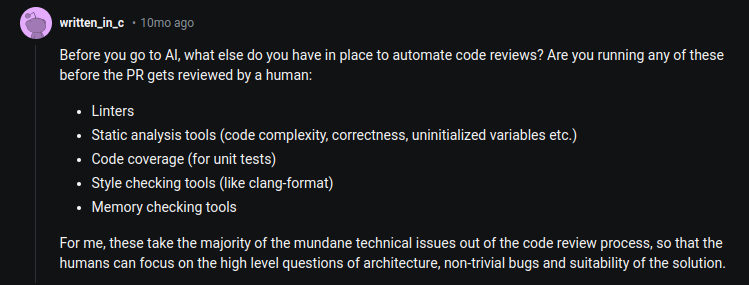
\includegraphics[width=0.8\textwidth]{./img/reddit.png}
    % \caption{}
    \label{fig:reddit_response}
\end{figure}

Herramientas de feedback de código gratuitas:

\begin{itemize}
    % \item \href{https://www.codefactor.io/}{CodeFactor}
    % \item \href{https://www.codacy.com/}{Codacy}
    % \item \href{https://www.codeclimate.com/}{CodeClimate}
    % \item \href{https://www.gitguardian.com/}{GitGuardian}
    % \item \href{https://www.sonarqube.org/}{SonarQube}
    \item \href{https://www.deepsource.com/}{DeepSource}
    \item \href{https://marketplace.visualstudio.com/items?itemName=SonarSource.sonarlint-vscode}{SonarLint}
    \item \href{https://marketplace.visualstudio.com/items?itemName=usernamehw.errorlens}{ErrorLens}
    \item \href{https://marketplace.visualstudio.com/items?itemName=CodeScene.codescene-vscode}{CodeScene}
\end{itemize}


\subsection{\href{https://www.ox.ac.uk/students/academic/guidance/skills/ai-study}{Use of generative AI tools to support learning}}

Blog acerca de recomendaciones de uso de AI para estudiantes de la Universidad de Oxford.

\section{Resumen}

\begin{center}
    \begin{table}
        \centering
        \begin{tabular}{|p{5cm}|p{3cm}|p{4cm}|}
        \hline
        Tecnicas & Experimentacion & Validacion \\ \hline
        Plugin de editor de texto, GitHub Action, Multiples agentes de AI &  A/B Testing limitando el espectro de errores a corregir               & number of code smells, code review participation, code review time, defect density, code quality improvement, number of refactored code smells, number of issues identified, media de issues detectados en cada code review, issues detectados por severidad (trivial, medium, critical)           \\ \hline
                    % &                 &            \\ \hline
        \end{tabular}
    \end{table}
\end{center}

\bibliographystyle{plain}
\bibliography{bibliography}


\end{document}

% https://tug.ctan.org/info/undergradmath/undergradmath.pdf
% https://github.com/jeremy-jmc/CS4054-Net/blob/main/labs/l4/informe/main.tex